% VUT FIT MITAI
% MSZ 2021/2022
% Author: Vladimir Dusek
% Login: xdusek27

%%%%%%%%%%%%%%%%%%%%%%%%%%%%%%%%%%%%%%%%%%%%%%%%%%%%%%%%%%%%%%%%%%%%%%%%%%%%%%%%

% Path to figures
\graphicspath{{pdi/map_reduce/figures}}

%%%%%%%%%%%%%%%%%%%%%%%%%%%%%%%%%%%%%%%%%%%%%%%%%%%%%%%%%%%%%%%%%%%%%%%%%%%%%%%%

\chapter{PDI -- Principy distribuovaného zpracování MapReduce, průběh a jednotlivé operace distribuovaného výpočtu pomocí MapReduce, jeho implementace v~Apache Hadoop a Apache Spark.}

%%%%%%%%%%%%%%%%%%%%%%%%%%%%%%%%%%%%%%%%%%%%%%%%%%%%%%%%%%%%%%%%%%%%%%%%%%%%%%%%

\section{Metadata}

\begin{compactitem}
    \item Předmět: Prostředí distribuovaných aplikací (PDI)
    \item Přednáška:
    \begin{compactitem}
        \item 9) Programovací model MapReduce a Apache Hadoop
        \item 10) Distribuované souborové systémy
        \item 11) Apache Spark
    \end{compactitem}
    \item Záznam:
    \begin{compactitem}
        \item 2020-11-16
        \item 2020-11-23
    \end{compactitem}
\end{compactitem}

%%%%%%%%%%%%%%%%%%%%%%%%%%%%%%%%%%%%%%%%%%%%%%%%%%%%%%%%%%%%%%%%%%%%%%%%%%%%%%%%

\section{Úvod a kontext}

\paragraph*{OLTP} OLTP (\textit{Online Transactional Processing}, provozní databáze, systémy pro online zpracování transakcí) jsou standardní databázové systémy s~pevnou strukturou dat definovou pomocí databázového schématu. Jsou navrženy a optimalizovány pro chod provozních aplikací s~primárním cílem zajistit rychlý a souběžný přístup k~datům. To vyžaduje transakční zpracování, řízení souběžnosti a techniky obnovy (rollback), které zaručují konzistenci dat. Díky těmto vlastnostem mají OLTP databáze špatný výkon při provádění složitých dotazů, které potřebují spojit mnoho relačních tabulek dohromady nebo agregovat velké objemy dat. Kromě toho obsahují typicky podrobná data a neobsahují historická data, která jsou při datové analýze potřeba.

\paragraph*{OLAP} OLAP (\textit{Online Analytical Processing}, online analytické zpracování) je databázové paradigma specificky zaměřené na dotazy, zejména na analytické dotazy. Používají se zde jiné techniky indexování a optimalizace dotazů. Normalizace není pro toto paradigma žádoucí, protože rozděluje databázi na mnoho tabulek. Složité dotazy v~takovém případě vyžadují rekonstrukci dat a s~tím spojený vysoký počet spojování tabulek. Pracuje se s~tzv. multidimenzionálními kostkami, avšak v~pozadí jsou stále relační databáze.

\paragraph*{NoSQL} Potřeba ukládat proudy dat (zpracovávané v~reálném čase bez možnosti pozastavení), obrázky, multimédia, velké JSON soubory, \dots, vedla ke vzniku NoSQL databází. NoSQL databáze používají jiné prostředky než tabulková schémata tradiční relační databáze. Často jde o~\uv{hloupé}, nestrukturované uložiště klíč-hodnota.

\paragraph*{BigData} Velká, nestrukturovaná (různorodá), rychle rostoucí data, která není možné uložit ani zpracovávat běžnými přístupy (na jednom uzlu, jedním uzlem). Produkují je např.: IoT senzory, sociální sítě, chatovací aplikace, webové vyhledávače, \dots \, Pro jejich zpracování je nutné využít distribuované systémy (pro uložení i zpracování).

\paragraph*{Distribuované zpracování dat} Distribuované zpracování dat je zpracování velkých dat (\textit{big data}) pomocí distribuovaných systémů. To s~sebou přináší problémy. Jak zaručit vhodnou distribuci dat a výpočtu mezi uzly? Jak řešit nespolehlivost a výpadky uzlů? Jak a kam zajistit doručení výsledků výpočtu? \dots

%%%%%%%%%%%%%%%%%%%%%%%%%%%%%%%%%%%%%%%%%%%%%%%%%%%%%%%%%%%%%%%%%%%%%%%%%%%%%%%%

\section{MapReduce}

Algoritmy pro indexování webových stránek (Page Rank) přestávaly být udržitelné, bylo potřeba zvýšit jejich škálovatelnost. Google vydal příspěvek \uv{MapReduce: Simplified Data Processing on Large Clusters}, kde bylo představeno paradigma MapReduce. Jde o~paradigma distribuovaného výpočtu založené na funkcích \textit{map} a \textit{reduce} z~funcionálního programování.

\paragraph*{Map} Funkce \textit{map} má ve funkcionálním programování 2 vstupní parametry a vrací seznam hodnot. První parametr je unární operátor (nebo funkce fungující jako unární operátor) a druhý je seznam hodnot. Výstupní seznam je spočítán jako aplikace unárního operátoru na vstupní seznam. Příklad:
$$
map(square, [1, 2, 3, 4]) = [1, 4, 9, 16]
$$.
V~paradigmata MapReduce \textit{map} vrací data jako seznam dvojic klíč-hodnota, přesněji: $$
map((key, value)) \rightarrow [(key, value)]
$$.

\paragraph*{Reduce} Funkce \textit{reduce} má ve funkcionálním programování 2 vstupní parametry a vrací jednu hodnotu. První parametr je binární operátor (nebo funkce fungující jako binární operátor) a druhý je seznam hodnot. Výstupní hodnota je spočítána jako postupná aplikace binárního operátoru na všechny hodnoty ve vstupním seznamu. Příklad:
$$
reduce(+, [1, 4, 9, 16]) = 30
$$.
V~paradigmata MapReduce \textit{reduce} bere na vstupu klíč a seznam hodnot a vrací opět seznam dvojic klíč-hodnota, přesněji: $$
reduce(key, [value]) \rightarrow [(key, value)]
$$.

\bigskip\noindent\begin{minipage}{\linewidth}
\begin{lstlisting}[language=Python, caption={Příklad implementace funkcí \textit{map} a \textit{reduce} v~paradigmatu MapReduce pro počítání četnosti slov ve vstupu v~Pythonu.}]
def map(input_key: str, input_value: str) -> list[tuple[str, int]]:
    # input_key - document name
    # input_value - document content (etc. line)
    result = []
    for word in input_value.split(' '):
        result.append((word, 1))
    return result

def reduce(input_key: str, input_value: list[int]) -> tuple[str, int]:
    result = 0
    for val in input_value:
        result += value
    return (input_key, result)
\end{lstlisting}
\end{minipage}

\begin{figure}[H]
    \centering
    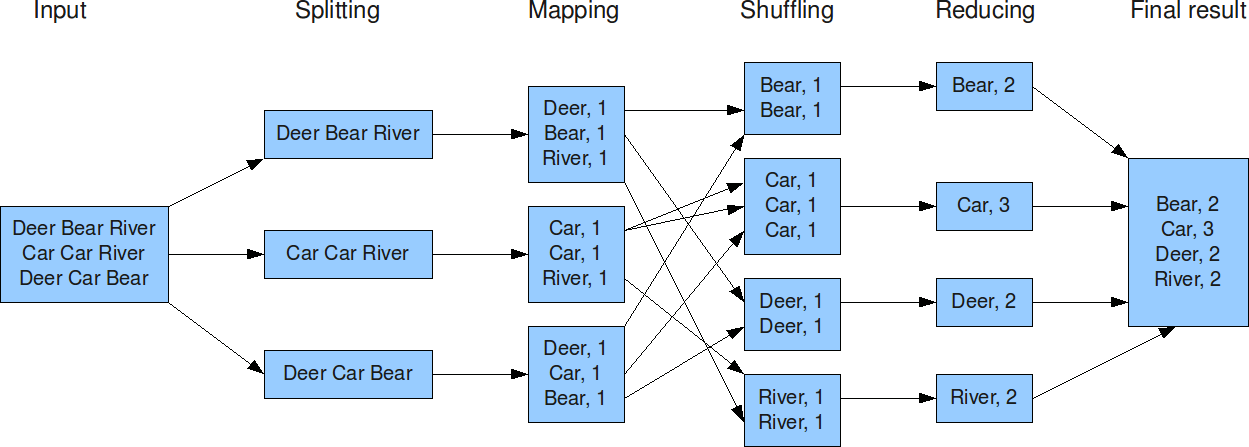
\includegraphics[width=1\linewidth]{map_reduce_example.png}
    \caption{Úloha počítání četnosti slov v~paradigmatu MapReduce v~diagramu.}
    \label{49_map_reduce_example}
\end{figure}

\paragraph*{Průběh MapReduce} Celý MapReduce probíhá v~několika krocích, viz obrázek~\ref{49_map_reduce_example}.
\begin{compactenum}
    \item Input -- Přípravený vstup pro distribuovaný výpočet (např. soubory ve virtuálním distribuovaném souborovém systému, viz dále HDFS).
    \item Splitting -- Rozdělení vstupu na části, které budou přiděleny jednotlivým uzlům. Může být výchozí (např. rozdělení textového souboru po řádcích) nebo definováno uživatelem.
    \item Mapping -- Každý uzel aplikuje funkci \textit{map} na svoji přidělenou část. Uživatel definuje jak má funkce \textit{map} vypadat.
    \item Shuffling (také Grouping, Partitioning, Comparing)-- Výpočetní uzly si mezi sebou vymění hodnoty, které spočítaly, na základě klíče. Tento krok zařižuje platforma pro distribuovaný výpočet sama o~sobě, typicky na základě hashů klíčů. Tento krok je většinou \textit{bottleneck}.
    \item Reducing -- Každý uzel zapojený do tohoto kroku (často je v~tomto kroku potřeba méně uzlů, než v~kroku mapping) aplikuje funkci \textit{reduce} na svoji přidělenou část. Uživatel definuje jak má funkce \textit{reduce} vypadat.
    \item Final Result -- Finální výsledek (např. zapsán do do virtuálního distribuovaného souborového systému, viz dále HDFS).
\end{compactenum}

\begin{figure}[H]
    \centering
    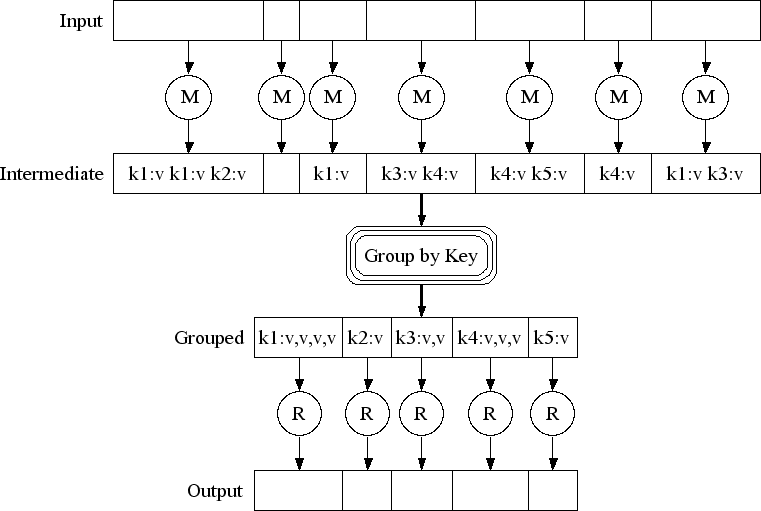
\includegraphics[width=1\linewidth]{map_reduce_general_p1.png}
    \caption{Výpočet MapReduce v~obecném schématu.}
\end{figure}

\paragraph*{Combiner} Optimalizační krok, jde o~\uv{jakési} provedení operace \textit{reduce} už ve fázi \textit{map} (každým uzlem). Tím je snížen počet mezivýsledků ve fázi Shuffling. Typicky funkce \textit{combine} je stejná jako \textit{reduce}.

\paragraph*{Virtuální distribuovaný souborový systém} Pro realizaci distribuovaného výpočtu je rovněž potřeba distribuovaný souborový systém (DFS). Ten je typicky realizován jako virtuální souborový systém nad jednotlivými souborovými systémy uzlů. Např.: GFS -- Google File System, HDFS -- Hadoop File System (viz dále). DFS obsahuje data samotná (\textit{data nodes}) a metadata o~tom, která data jsou na jakých uzlech (\textit{name nodes}).

\begin{figure}[H]
    \centering
    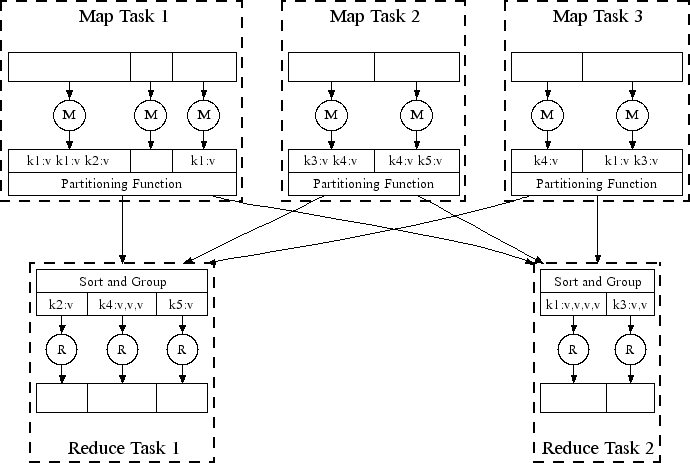
\includegraphics[width=1\linewidth]{map_reduce_general_p2.png}
    \caption{Výpočet MapReduce v~obecném schématu a rozdělením práce na jednotlivé uzly (uzel je typicky víceprocesorový).}
\end{figure}

%%%%%%%%%%%%%%%%%%%%%%%%%%%%%%%%%%%%%%%%%%%%%%%%%%%%%%%%%%%%%%%%%%%%%%%%%%%%%%%%

\section{Apache Hadoop}

% Todo:
% - Dale by se dalo mluvit podrobneji o implementaci, viz slajd 26 (job tracker, task tracker).

Apache Hadoop je \textit{open-source} implementace MapReduce paradigmatu vyvíjená Apache Software Foundation. Jde o~implementaci v~Jave, ta je vhodná, jelikož díky JVM (Java Virtual Machine) je spouštění uživatel definovaných funkcí \textit{map} a \textit{reduce} snadné.

\paragraph*{Hadoop MapReduce} -- Implementace MapReduce paradigma. Data jsou čtena a ukládána na HDFS (včetně mezivýsledků). To znamená, můžeme pracovat v~podstatě neomezenými daty, ale ukládání a načítání výpočet zpomalují.\footnote{\textit{Nebylo přednášeno podrobněji, pravděpodobně stačí princip obecného MapReduce, který byl vysvětlen v~předchozí sekci.}}.

\paragraph*{HDFS} HDFS (\textit{Hadoop Distribute File System}) je virtuální distribuovaný souborový systém. Standardní soubor je rozdělen na datové bloky které jsou distribuovány na různé datové uzly. Architektura HDFS se skládá ze dvou typů uzlů~--~Name Node a Data Node. Name Node obsahuje alokační tabulku pro souborový systém. Ví které datové bloky patří kterému souboru a kde jsou uloženy. Obsahuje další metadata jako názvy souborů, cesty, \dots \, Data Node obsahuje datové bloky. Typicky redundance a replikace, počítá se s~možným selháním uzlů. Pro \textbf{čtení dat} se klient zeptá Name Nodu na konkrétní soubor v~HDFS. Name Node vrátí metadata o~souboru, na jakých Data Nodech se vyskytuje. Klient požádá příslušné Data Nody, ty mu pošlou data, která se na klientovi \uv{poskládají} do výsledného souboru. Pro \textbf{zápis dat} se klient zeptá Name Nodu, kam by měl zapisovat. Klient zapíše na příslušný Data Node. Data Node poté vyřeší replikace s~dalšími uzly.

\paragraph*{Hadoop YARN} Hadoop YARN je plánovač (\textit{scheduler}). Plánuje výpočet tak, aby proběhl co nejlepším způsobem na konkrétnbí distribuované architektuře. Plánovač má obecné obecné rozhraní a Hadoop YARN lze nahradit za jiný.

\paragraph*{Hadoop Common} Hadoop Common jsou další knihovny a ovladače pro klienty.

\paragraph*{Další nástroje} Nad Apache Hadoop existuje mnoho dalších nástrojů. Apache Pig pro \textit{high level} programování map-reduce úloh. Apache Hive pro pro dolování dat nad Apache Hadoop. Apache HBase jako distribuovaná databáze nad Apache Hadoop, \dots

%%%%%%%%%%%%%%%%%%%%%%%%%%%%%%%%%%%%%%%%%%%%%%%%%%%%%%%%%%%%%%%%%%%%%%%%%%%%%%%%

\section{Apache Spark}

Apache Spark je \textit{open-source} nástroj pro distribuované zpracování rozsáhlých dat vyvíjený Apache Software Foundation. Hlavní cíl je zvýšení rychlosti. Spark na to jde přesunutím co nejvíce výpočtů do operační paměti jednotlivých uzlů a tím pádem zminimalizovat počet zápisů a čtení z~DFS (snaha odstranit \textit{bottleneck} v~kroku shuffling u~Hadoopu). Tím ale vzniká jiný problém, a sice výpadek uzlu znamená, že data jsou ztraceny.

\begin{figure}[H]
    \centering
    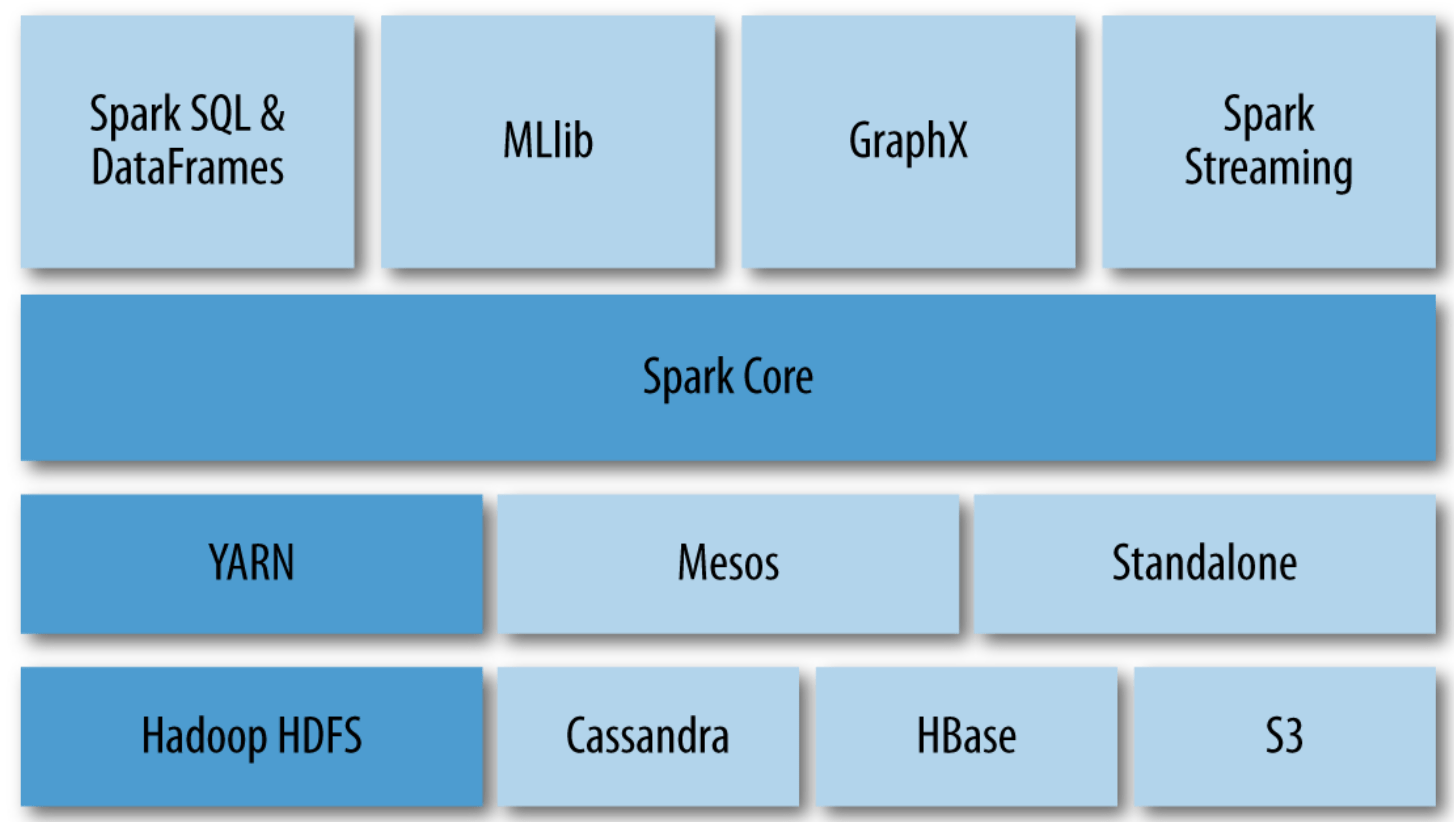
\includegraphics[width=0.75\linewidth]{spark.png}
    \caption{Architektura Apache Spark. Hlavní je Spark Core, zbytek funguje na systému pluginů a může používat HDFS, Hadoop YARN a Hadoop Common.}
\end{figure}

% todo: pokracovani, 30 min prednaska

\paragraph*{Resilient Distributed Dataset} Resilient Distributed Dataset (RDD) je základní datová struktura Sparku. Jedná se o~typované kolekce n-tic, které jsou neměnné (\textit{read only}). Vstup je transformován na RDD a každá operace je pak transformace jednoho RDD na jiné.
$$
RDD_1 \rightarrow map() \rightarrow RDD_2 \rightarrow reduce() \rightarrow RDD_3
$$

\paragraph*{Strategie vyhodnocování} Spark uplatňuje strategii vyhodnocování \textit{lazy evaluation}. Vyhodnocování výrazu je odkládáno až do doby, dokud není potřeba jeho hodnota. Zabraňuje opakovanému vyhodnocování. Je vyhodnocována pouze ta část, která je potřeba. RDD funguje jako abstraktní datová struktura, nemusí obsahovat data uvnitř, ale pouze předpis jak data získat a získá je, až když jsou potřeba.

\paragraph*{Struktura výpočtu} Struktura výpočtu odpovídá orientovanému acyklickému grafu (DAG, \textit{Directed Acyclic Graph}). Uzly jsou RDD a hrany jsou transformace. DAG je znám i dalším uzlům, takže pokud nastane výpadek uzlu a výpočet je ztracen, může být uzel snadno zastoupen.

\paragraph*{Klíčové vlastnosti} Klíčové vlastnosti Sparku jsou \textit{lazy evaluation}, \textit{in-memmory} a \textit{parallel computing}.

\begin{figure}[H]
    \centering
    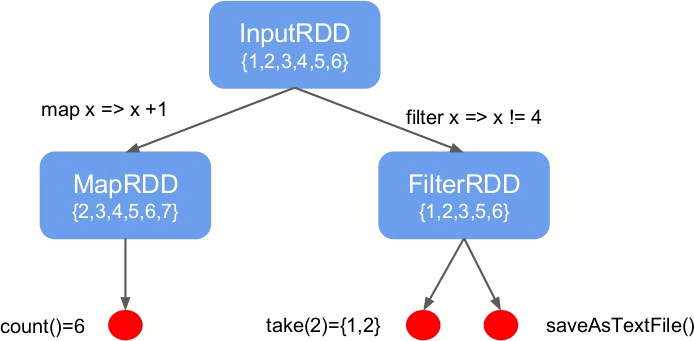
\includegraphics[width=0.85\linewidth]{spark_example.png}
    \caption{Příklad výpočtu v~Apache Spark.}
\end{figure}
